\documentclass[11pt]{article}
\usepackage{graphicx}
\usepackage{float}
\graphicspath{{figs/}}
    \DeclareGraphicsExtensions{.pdf,.jpg,.png,.eps}
\usepackage{subcaption}    
\usepackage{amsmath}
\usepackage{amssymb}
\usepackage{tikz}

\newcommand{\ie}{\textit{i.e.}}
%\newcommand{\st}{\textit{s.t.}}
\newcommand{\eg}{\textit{e.g.}}
\newcommand{\etc}{\textit{etc}}
\newcommand{\etal}{\textit{et~al.}} 
 
%% references
\newcommand{\secref}[1]{Sec.~\ref{#1}}
\newcommand{\dref}[1]{Definition~\ref{#1}}
\newcommand{\lemref}[1]{Lemma~\ref{#1}}
\newcommand{\thmref}[1]{Theorem~\ref{#1}}
\newcommand{\equref}[1]{Eq.~\ref{#1}}
\newcommand{\algmref}[1]{Algorithm~\ref{#1}}
%\newcommand{\cref}[1]{{\citet{#1}}}
\newcommand{\figref}[1]{Fig.~\ref{#1}}
\newcommand{\subfig}[1]{\textit{#1}}
\newcommand{\tabref}[1]{Table~\ref{#1}}
\newcommand{\prfref}[1]{Proof~\ref{#1}}
\newcommand{\asmref}[1]{Assumption~\ref{#1}} 
 
 
\title{Predicting Human Trust in Robot Capabilities across Tasks: Supplementary Material}
\author{Harold Soh, Pan Shu, Min Chen, and David Hsu}   
    
\begin{document}
\maketitle
\section{Autonomous Driving Experiment Setup}
\label{sec:driving-setup}

An overview of the experiment setup is shown in~\figref{fig:driving-task}. 
The participant interacted with a driving simulator 
built on Unity 3D engine. 
The robot car was controlled using the hybrid A* search algorithm and a proportional-integral-derivative (PID) controller.
The participant played the role of a safety driver, \ie, the participant only intervened if he/she believed the autonomous car would crash into something. Otherwise, the participant simply observed the autonomous vehicle.


\begin{figure}
    \centering
    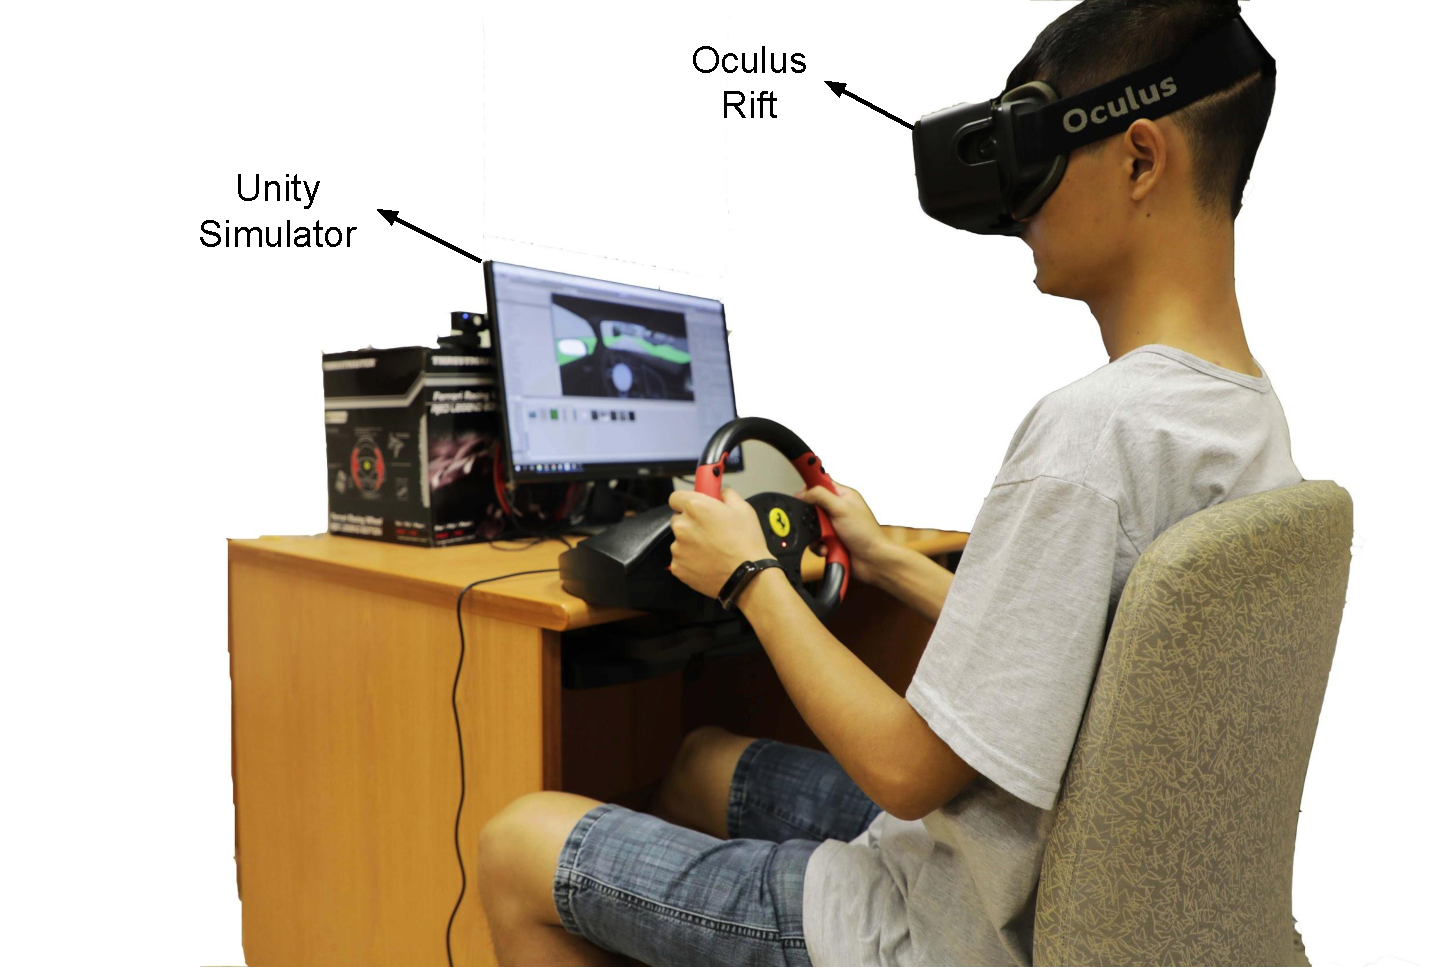
\includegraphics[width=.9\columnwidth]{figs/driving-setup.pdf}
    \caption{Autonomous driving experiment setup.}
    \label{fig:driving-task}
\end{figure}


Variable robot performance was controlled by our algorithm. At each trail of interaction, we intentionally let the robot car succeed or fail to see how participant's trust evolves after seeing the robot performance. For example,
\figref{fig:variable-success-failure} shows the pre-programmed robot  success/failure cases in the lanemerge task and parking forwards task.

\begin{figure}
    \centering
    \begin{tabular}{c c}
        \centering
        \begin{subfigure}{.48\columnwidth}
            \centering
            \begin{tabular}{cc}
                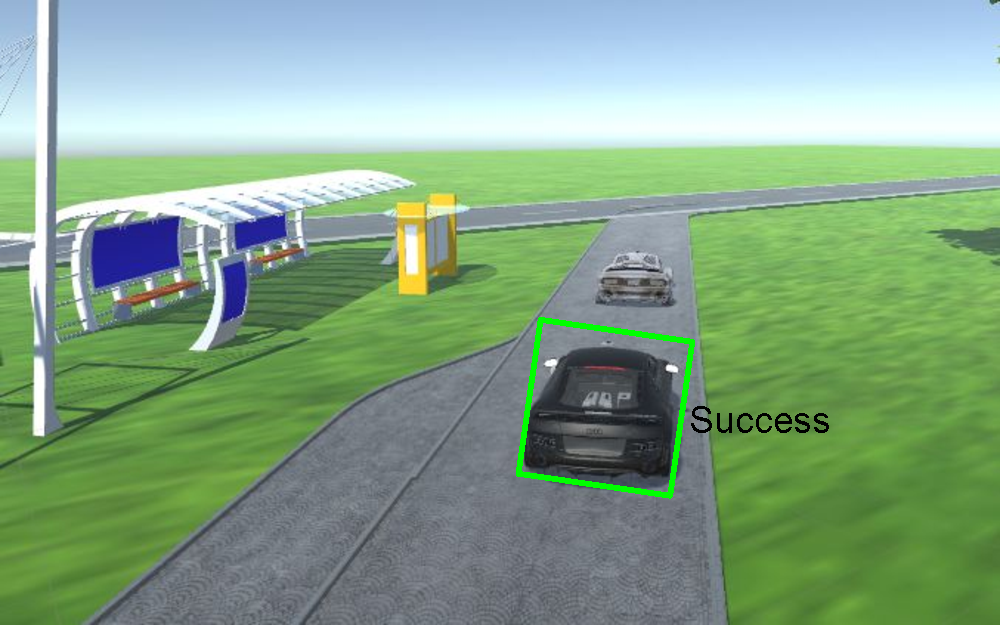
\includegraphics[width=0.9\linewidth]{figs/driving-text/lanemerge-success.pdf}
                \\
                \\
                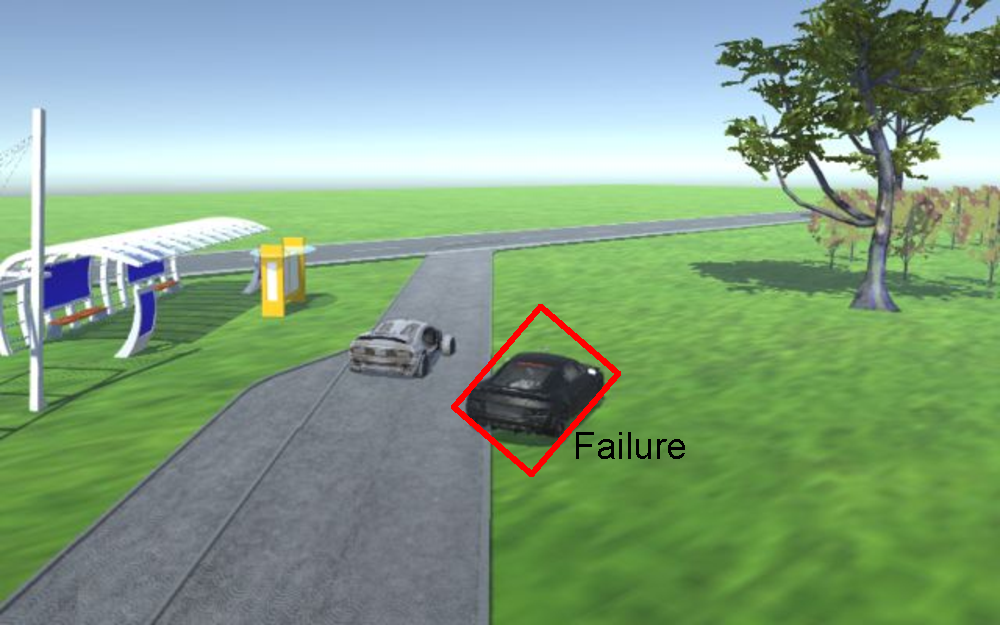
\includegraphics[width=0.9\linewidth]{figs/driving-text/lanemerge-failure.pdf}
            \end{tabular}
        \end{subfigure}

        \hspace{10pt}

        \begin{subfigure}{.48\columnwidth}
            \centering
            \begin{tabular}{cc}
                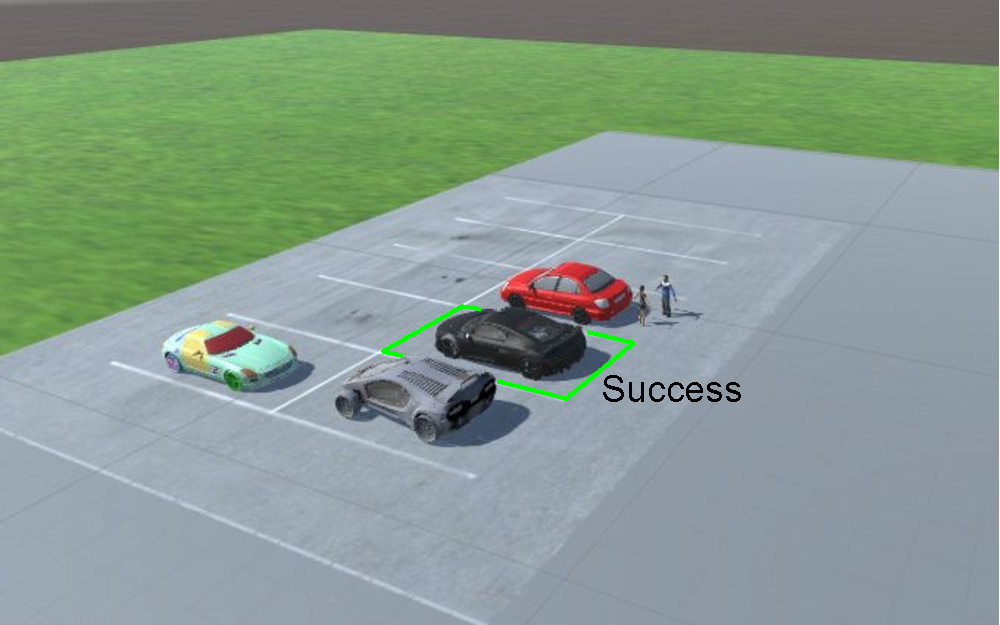
\includegraphics[width=0.9\linewidth]{figs/driving-text/parking-success.pdf}
                \\
                \\
                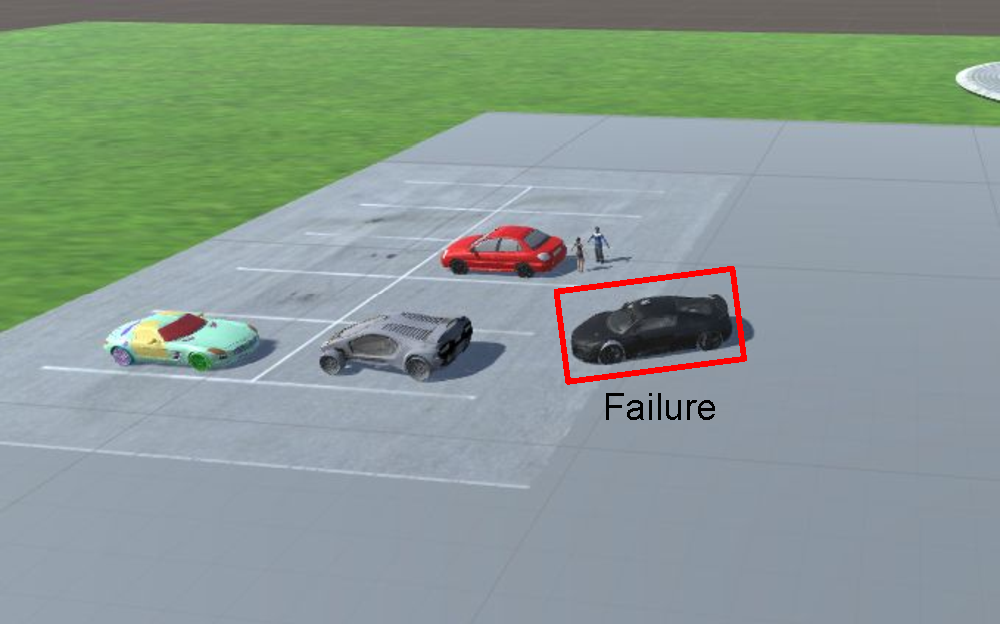
\includegraphics[width=0.9\linewidth]{figs/driving-text/parking-failure.pdf}
            \end{tabular}
        \end{subfigure}
    \end{tabular}
    \caption{Robot car success/failure in the lane merge task (left column). 
        Robot car success/failure in the parking forwards task (right column).}
    \label{fig:variable-success-failure}
\end{figure}
\end{document}
